

\documentclass[11pt]{article}


%%%%%%%%%%%%%%%
\def\Type{ApplicationPreDJ}
\def\TypeNum{Pre-class for Application Day: Gradient Descent Method}
\def\TypeTitle{Gradient Descent}
\def\Semester{Fall 2025}
\def\Course{Math 1190/1210}
%\def\Targets{{\bf\color{Goldenrod}AD1}}
\def\desmosClassCode{{\bf ZAJ$3$AZ}}
\usepackage{preambleDJ}
\usepackage{graphicx}
\usepackage{footnote}
\usepackage{tikz}
\usepackage{pgfplots}
\usepackage[colorlinks=true, linkcolor=blue, urlcolor=blue]{hyperref}
\pgfplotsset{compat=1.18}  % adjust to your version
\makesavenoteenv{minipage}
\begin{document}
%!TEX TS-program = xelatex
%!TEX encoding = UTF-8 Unicode



\pagestyle{otherpages}
\thispagestyle{firstpage}
\vspace*{.65in}
%If Ada Lovelace\footnote{\url{https://en.wikipedia.org/wiki/Ada_Lovelace}} is the ``mother of programming" then 
{\bf Introduction}\\

\noindent
\begin{minipage}[c]{0.35\textwidth}
    \centering
    
\includegraphics[width=\linewidth]{Spring 2026/ApplicationDays/GradientDescent/images/feiFeiLiWiredCropped.png}
\end{minipage}
\hspace{0.02\textwidth}
\begin{minipage}[c]{0.63\textwidth}
Fei-Fei Li is known as the ``godmother of A.I'' for her groundbreaking contributions in computer vision and deep learning and as the creator of ImageNet\footnote{
See ``Godmother of A.I." Fei-Fei Li on technology development: ``The power lies within people" at \url{https://www.cbsnews.com/news/godmother-of-a-i-on-technology-development-fei-fei-li/}\\
or Britannica at \url{https://www.britannica.com/biography/Fei-Fei-Li}, The Guardian \href{https://www.theguardian.com/technology/2023/nov/05/ai-pioneer-fei-fei-li-im-more-concerned-about-the-risks-that-are-here-and-now}{\underline{here}} or \url{https://en.wikipedia.org/wiki/Fei-Fei_Li}
}.

\vspace{1em}

In this application, we will be exploring how the Gradient Descent method can be used for a supervised machine learning model that we have already seen in the Keeling Curve application. But before we do that, we need to refresh our memories about some properties of derivatives.

\medskip
{\bf Example 1: Function and Derivative}\\

Consider the function
\[
f(x) = x^2
\]

\begin{enumerate}
\item Compute the derivative:
\[
f'(x) = \rule{5cm}{0.4pt}
%\unline{1}{\blue{2x}}{.25}
\]

\item Evaluate at $x=3$:
\[
f'(3) = \rule{5cm}{0.4pt}
%\unline{1}{\blue{6}}{.25}
\]

\item Interpretation: since $f'(3) > 0$, the slope is positive. To decrease the value of $f(x)$ to be smaller than $f(3) = 9$, we should move to the left (decrease $x$) to go toward a smaller number. 
\end{enumerate}
\medskip
% Graph of f(x) = x^2 and tangent at x=3 with grid
\begin{center}
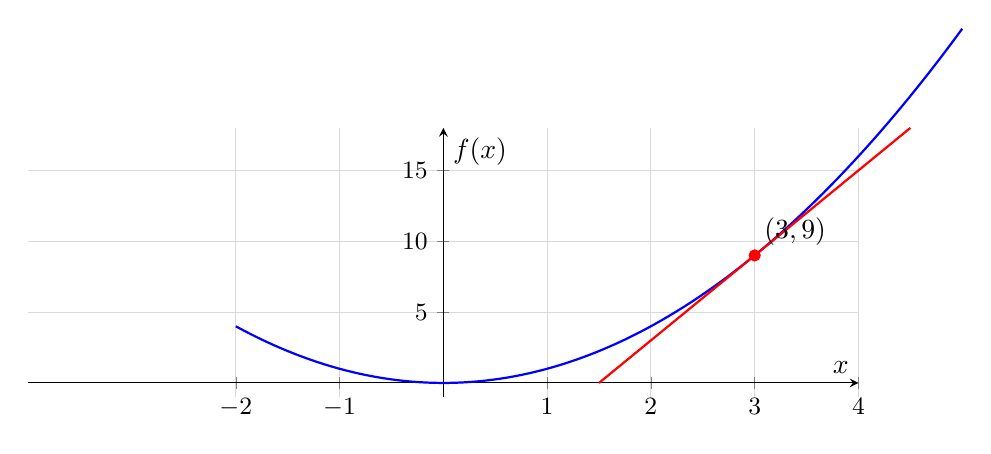
\begin{tikzpicture}
\begin{axis}[
    width=\linewidth,       % use full width of the minipage
    height=5cm,             % adjust height as needed
    axis lines=middle,
    xlabel=$x$, ylabel=$f(x)$,
    xmin=-4, xmax=4,
    ymin=-1, ymax=18,
    xtick={-2,-1,0,1,2,3,4},
    ytick={0,5,10,15,20},
    grid=both,              % add grid lines
    grid style={gray!30},   % light gray grid
    tick label style={font=\small}, % smaller labels
    enlargelimits=false,
    clip=false
]

% f(x) = x^2
\addplot [domain=-2:5, samples=100, blue, thick] {x^2};

% Tangent at x=3: f'(3) = 6
\addplot [domain=1.5:4.5, red, thick] {6*(x-3)+9};

% Mark the point (3,9)
\addplot[only marks, mark=*, red] coordinates {(3,9)};
\node[above right] at (axis cs:3,9) {$(3,9)$};

\end{axis}
\end{tikzpicture}
\end{center}
\end{minipage}
\newpage
\textbf{Moving Along the Slope (Gradient Descent Intuition):} \\
Suppose we want to find the minimum of a twice differentiable function $f(x)$.
\begin{itemize}
    \item At a point $x_{\text{old}}$, the slope of the tangent line to the graph of the function $f(x)$ at the point $x_{\text(old)}$ is the value (or number) $f'(x_{\text{old}})$.
    \item If $f'(x_{\text{old}}) > 0$, the original function $f(x)$ is increasing in some small open interval around $x_{\text{old}}$, so move \emph{left} (in the negative direction) along the $x$-axis (decrease $x$) to decrease the $y-value$ (i.e. to go downhill).
    \item If $f'(x_{\text{old}}) < 0$, the original function $f(x)$ is decreasing in some small open interval around $x_{\text{old}}$, so move \emph{right} (in the positive direction) along the $x$-axis (decrease $x$) to decrease the $y-value$ (i.e. to go downhill).
    \item The new point is
    \[
    x_{\text{new}} = x_{\text{old}} - \alpha f'(x_{\text{old}}),
    \]
    where $\alpha>0$ is the caled the\emph{step size}, and controls how far we move.
\end{itemize}

\begin{figure}[h!]
\centering
\begin{minipage}{0.45\textwidth}
\centering
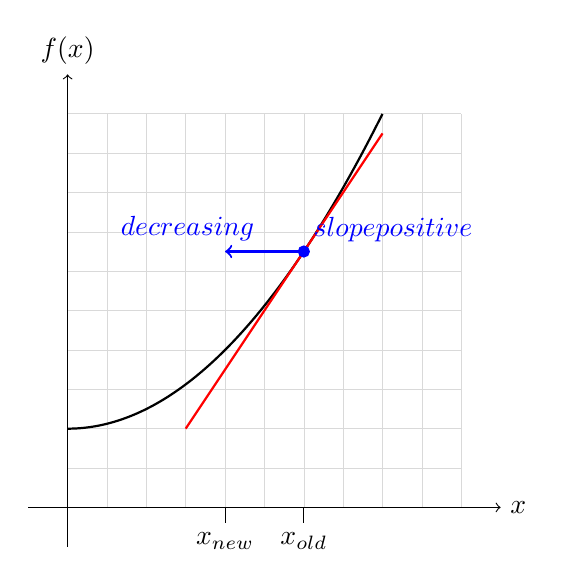
\begin{tikzpicture}[scale=1.0]
    % grid
    \draw[step=0.5, gray!30, very thin] (0,0) grid (5,5);
    
    % axes
    \draw[->] (-0.5,0) -- (5.5,0) node[right] {$x$};
    \draw[->] (0,-0.5) -- (0,5.5) node[above] {$f(x)$};
    
    % function
    \draw[thick, domain=0:4, samples=100, smooth] plot (\x,{0.25*\x*\x+1});
    
    % tangent line through x=3
    \draw[red, thick, domain=1.5:4] plot (\x,{1.5*\x -1.25}); % tangent using slope f'(3)=3
    
    % point on curve
    \filldraw[blue] (3,3.25) circle (2pt) node[above right] {$\text{slope positive}$};
    
    % gradient descent arrow
    \draw[->, thick, blue] (3,3.25) -- (2,3.25) node[midway, above left] {$\text{decreasing }$};
    
    % x labels
    \draw (3,0) -- (3,-0.2) node[below] {$x_\text{old}$};
    \draw (2,0) -- (2,-0.2) node[below] {$x_\text{new}$};
\end{tikzpicture}
\caption*{Slope $f'(x_\text{old})>0$: move left along $x$ to decrease $f(x)$.}
\end{minipage}
\hfill
\begin{minipage}{0.45\textwidth}
\centering
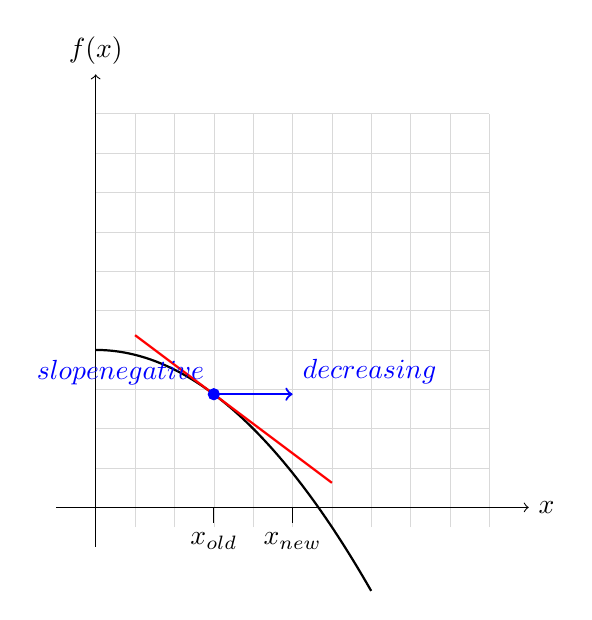
\begin{tikzpicture}[scale=1.0]
    % grid
    \draw[step=0.5, gray!30, very thin] (0,-0.25) grid (5,5);
    
    % axes
    \draw[->] (-0.5,0) -- (5.5,0) node[right] {$x$};
    \draw[->] (0,-0.5) -- (0,5.5) node[above] {$f(x)$};
    
    % function
    \draw[thick, domain=0:3.5, samples=100, smooth] plot (\x,{-0.25*\x*\x+2});
    
    % tangent line through x=1.5
    \draw[red, thick, domain=0.5:3] plot (\x,{-0.75*\x + 2.5625}); % tangent f'(1.5)=1.5
    
    % point on curve
    \filldraw[blue] (1.5,1.4375) circle (2pt) node[above left] {$\text{slope negative}$};
    
    % gradient descent arrow
    \draw[->, thick, blue] (1.5,1.4375) -- (2.5,1.4375) node[above right] {$\text{decreasing}$};
    
    % x labels
    \draw (1.5,0) -- (1.5,-0.2) node[below] {$x_\text{old}$};
    \draw (2.5,0) -- (2.5,-0.2) node[below] {$x_\text{new}$};
\end{tikzpicture}
\caption*{Slope $f'(x_\text{old})<0$: move right along $x$ to decrease $f(x)$.}
\end{minipage}
\end{figure}

\emph{In other words: we slide down the graph of the function along the tangent line, moving in the direction (positive or negative direction of the number line) that is opposite to the sign of the slope at our current point.}
%%%%%%%%%%%%%%%%%%%%%%%%%%%%%%%%%%%%%%%%%%%%%%%%%%%%%%%%%%%%%%%%%%%%%%%%%%%%%%%%%%%%%%%%%%%%%%%%%%%%%%%%%%%%%%%%%%%%%%%%%%%%%%%%%%%%%%%%%%%%%%%%%%%%%%%%%%%%%%%%%%%%%%%%%%%%%%%%%%%%%%%%%%%%%%%%%%%%%%%%%%%%%%%%%%%%%%

\section*{Gradient Descent: Why it works}

Suppose we have a function $f(x)$ and we want to find a value of $x$ that \emph{minimizes} $f$.  

\subsection*{1. Slope at a Point}

At a point $x_{\text{old}}$, the slope of $f$ is given by the derivative:
\[
f'(x_{\text{old}}) = \lim_{\Delta x \to 0} \frac{f(x_{\text{old}}+\Delta x) - f(x_{\text{old}})}{\Delta x}.
\]
\begin{itemize}
\item If $f'(x_{\text{old}}) > 0$, the function is increasing at $x_{\text{old}}$.
\item If $f'(x_{\text{old}}) < 0$, the function is decreasing at $x_{\text{old}}$.
\end{itemize}


If $\Delta x$ is ``very small" we can formally clear fractions in the limit definition approximate the derivative as:
\[
f'(x_{\text{old}})\Delta x \approx f(x_{\text{old}}+\Delta x) - f(x_{\text{old}}).
\]



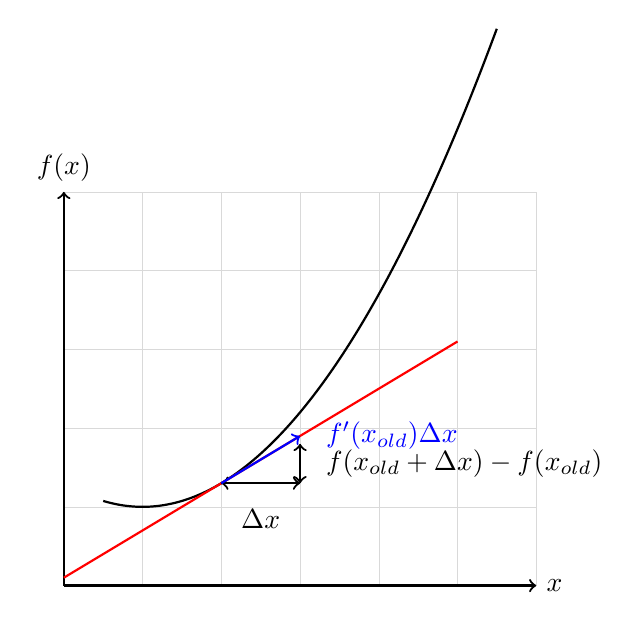
\begin{tikzpicture}[scale=1.0]

% Grid
\draw[gray!30, very thin] (0,0) grid (6,5);

% Axes
\draw[->, thick] (0,0) -- (6,0) node[right] {$x$};
\draw[->, thick] (0,0) -- (0,5) node[above] {$f(x)$};

% Function
\draw[thick, domain=0.5:5.5, samples=100, smooth] plot (\x,{0.3*(\x-1)^2+1});

% Points
\coordinate (xold) at (2,1.3);
\coordinate (xnew) at (3,1.8);

% Tangent line at x_old
\draw[red, thick, domain=0:5] plot (\x,{0.6*(\x-2)+1.3}); % slope f'(x_old)=0.6

% Points on function
%\filldraw[blue] (xold) circle (2pt) node[above left=4mm and 3mm] {$x_\text{old}, f(x_\text{old})$};
%\filldraw[blue] (xnew) circle (2pt) node[above right=4mm and 4mm] {$x_\text{old}+\Delta x, f(x_\text{old}+\Delta x)$};

% Vertical difference
\draw[dashed] (xold) -- (xnew |- xold);
\draw[<->, thick] (xnew |- xold) -- (xnew) node[midway, right=2mm] {$f(x_\text{old}+\Delta x)-f(x_\text{old})$};

% Horizontal difference
\draw[<->, thick] (xold) -- (xnew |- xold) node[midway, below=2mm] {$\Delta x$};

% Tangent slope label
\draw[->, blue, thick] (xold) -- ++(1,0.6) node[right=2mm] {$f'(x_\text{old})\Delta x$};

\end{tikzpicture}














\subsection*{2. Moving Opposite the Slope}

This means to \emph{decrease} $f$, we move in the direction opposite to the slope.  
If we move a small amount $\Delta x$, the tangent line gives a good approximation:
\[
f(x_{\text{old}} + \Delta x) \approx f(x_{\text{old}}) + f'(x_{\text{old}}) \Delta x.
\]




\subsection*{3. Updating the $x$-Value}

Using this step, we define the new $x$ value as:
\[
x_{\text{new}} = x_{\text{old}} + \Delta x = x_{\text{old}} - \alpha f'(x_{\text{old}}).
\]

Substituting $\Delta x$ into the linear approximation:
\[
f(x_{\text{new}}) \approx f(x_{\text{old}}) + f'(x_{\text{old}})(-\alpha f'(x_{\text{old}})) = f(x_{\text{old}}) - \alpha (f'(x_{\text{old}}))^2.
\]

Since both $\alpha$ and $(f'(x_{\text{old}}))^2 \ge 0$, we have
\[
f(x_{\text{new}}) < f(x_{\text{old}}),
\]
so each step moves us downhill.


\subsection*{Summary}

Gradient descent algorithm:

\begin{enumerate}
    \item Compute the slope $f'(x_{\text{old}})$ using the derivative.
    \item Move opposite the slope: $x_{\text{new}} = x_{\text{old}} - \alpha f'(x_{\text{old}})$.
    \item Repeat until $f'(x)$ is close to $0$.
\end{enumerate}

This method uses the limit definition of the derivative and the tangent line approximation to guide us to smaller function values.
%%%%%%%%%%%%%%%%%%%%%%%%%%%%%%%%%%%%%%%%%%%%%%%%%%%%%%%%%%%%%%%%%%%%%%%%%%%%%%%%%%%%%%%%%%%%%%%%%%%%%%%%%%%%%%%%%%%%%%%%%%%%%%%%%%%%%%%%%%%%%%%%%%%%%%%%%%%%%%%%%%%%%%%%%%%%%%%%%%%%%%%%%%%%%%%%%%%%%%%%%%%%%%%%%%%%%%\subsection*{Number of Steps in Gradient Descent}

In gradient descent, we update our estimate $x$ iteratively using:

\[
x_{\text{new}} = x_{\text{old}} - \alpha f'(x_{\text{old}})
\]

Here, $\alpha > 0$ is the \textbf{step size or learning rate}, controlling how far we move along the slope.
\textbf{Note:} A smaller $\alpha$ = smaller steps. A larger $\alpha$ = faster but can overshoot.
We do not jump to the minimum in one step because:
\begin{itemize}
    \item The slope may change along the curve.
    \item A large jump might overshoot the minimum.
    \item Small steps allow us to approximate the minimum gradually.
\end{itemize}

We repeat this update for a certain number of iterations, called the \textbf{number of steps}, denoted $n_\text{steps}$. Each step brings us closer to the minimum, and more steps generally result in a more accurate approximation:

\[
x_1 = x_0 - \alpha f'(x_0), \quad
x_2 = x_1 - \alpha f'(x_1), \quad
\ldots, \quad
x_{n_\text{steps}} = x_{n_\text{steps}-1} - \alpha f'(x_{n_\text{steps}-1})
\]



















\newpage
{\bf Gradient Descent Algorithm}\\
We can use the derivative to iteratively approach the minimum. Use our initial function $f(x) = x^2$ to find the mimimum value using the algorithm:

\[
x_{\text{new}} = x_{\text{old}} - \alpha f'(x_{\text{old}})
\]

\enum{

\item Let's take $x_0 = 3$ and $\alpha = 0.1$. Compute the first three iterations by hand:
\enum{
\item $x_1 = x_0 - (0.1) f'(x_0)$ = \rule{5cm}{0.4pt}  % 5 cm long, 0.4 pt thick
%3 - 0.1(6) = \unline{1}{\blue{2.4}}{.25}$
\vspace{4cm}

\item $x_2 = x_1 - (0.1) f'(x_1)$ = \rule{5cm}{0.4pt}  % 5 cm long, 0.4 pt thick
%2.4 - 0.1(4.8) = \unline{1}{\blue{1.92}}{.25}$
\vspace{4cm}

\item $x_3 = x_2 - (0.1) f'(x_2)$ \rule{5cm}{0.4pt}  % 5 cm long, 0.4 pt thick
%1.92 - 0.1 f'(1.92) = 1.92 - 0.1(3.84) = \unline{1}{\blue{1.536}}{.25}$
\vspace{4cm}

}

\item Apply gradient descent to $f(x) = (x-2)^2$ with $x_0 = 0$ and $\alpha = 0.2$. Compute the first 2 steps.
\newpage

\item Apply gradient descent to $f(x) = x^4 - 4x^2 + 3$ with $x_0 = 2$ and $\alpha = 0.05$. Compute the first 2 steps.
\vspace{4cm}

\item What happens if $\alpha$ is too big? Try to compute the first 3 steps with $\alpha = 1$ on $f(x) = x^2$ with $x_0 = 3$.
\vspace{4cm}

}

\section*{Gradient Descent Exploration Activity}

In this activity, you will use both calculus and an interactive app to explore how \textbf{gradient descent} finds minimum values of functions.

\subsection*{Part 1: Finding Minimums by Hand}

For each function below:

\begin{itemize}
    \item Compute $f'(x)$
    \item Find all critical points
    \item Determine which are minimums
\end{itemize}

\begin{enumerate}
    \item $f(x) = x^2$
    \begin{itemize}
        \item $f'(x)$ = \rule{5cm}{0.4pt} \\
        \vspace{1cm}
        
        \item \text{Critical Points} = \rule{5cm}{0.4pt} \\
        \vspace{1cm}

        \item \text{Minimums}  = \rule{5cm}{0.4pt} 
        \vspace{1cm}
        
    \end{itemize}

    \item $f(x) = e^x - x$
        \begin{itemize}
        \item $f'(x)$ = \rule{5cm}{0.4pt} \\
        \vspace{1cm}
        
        \item \text{Critical Points} = \rule{5cm}{0.4pt} \\
        \vspace{1cm}

        \item \text{Minimums}  = \rule{5cm}{0.4pt} 
        \vspace{1cm}
        
    \end{itemize}
    \item $f(x) = x^4 - 2x^2 + 1$
        \begin{itemize}
        \item $f'(x)$ = \rule{5cm}{0.4pt} \\
        \vspace{1cm}
        
        \item \text{Critical Points} = \rule{5cm}{0.4pt} \\
        \vspace{1cm}

        \item \text{Minimums} =  \rule{5cm}{0.4pt} 
        \vspace{1cm}
        
    \end{itemize}

    \item $f(x) = x^{1/3}$ \\
        \begin{itemize}
        \item $f'(x)$ = \rule{5cm}{0.4pt} \\
        \vspace{2cm}
        
        \item \text{Critical Points} = \rule{5cm}{0.4pt} \\
        \vspace{2cm}

        \item \text{Minimums} = \rule{5cm}{0.4pt} 
        \vspace{2cm}
        
    \end{itemize}
    \textit{(Can you find where $f'(x) = 0$? What is different about this function?)}
\end{enumerate}

\subsection*{Part 2: Exploring Gradient Descent}

Now open the Gradient Descent app. Found here: \href{https://woodword0-gradientdescentapplication.hf.space/}{Open the Gradient Descent App}


\begin{itemize}
    \item Select a function from the drop down menu
    \item Try different starting points $x_0$
    \item Try different learning rates $\alpha$
    \item Observe the sequence of points
\end{itemize}

\textbf{Answer the following questions:}

\begin{enumerate}

    \item For $f(x) = x^2$:
    \begin{itemize}
        \item Does gradient descent always find the minimum?
         \vspace{2cm}
        
        \item What happens if $\alpha$ is very large?
    \end{itemize}
    \vspace{2cm}

    \item For $f(x) = e^x - x$:
    \begin{itemize}
        \item Does the method converge to the same point from different starting values?
        \vspace{2cm}
        
        \item What do you notice about the slope near the minimum?
    \end{itemize}
    \vspace{2cm}

    \item For $f(x) = x^4 - 2x^2 + 1$:
    \begin{itemize}
        \item How many minimums does this function have?
         \vspace{2cm}
        
        \item Does gradient descent always find the same one?
         \vspace{2cm}
        
        \item How does the starting point affect the result?
    \end{itemize}
    \vspace{2cm}

    \item For $f(x) = x^{1/3}$:
    \begin{itemize}
        \item What happens near $x = 0$?
         \vspace{2cm}
        
        \item Does gradient descent behave differently here?
         \vspace{2cm}
        
        \item Why might this happen based on the derivative?
    \end{itemize}
    \vspace{2cm}

\end{enumerate}

\end{document}